
\section{Vorgehensmodell}%Thorsten
        Das Entwicklungsteam hat sich bei der Wahl des Vorgehensmodells \index{Vorgehensmodell} f\"ur das Modell der 
    evolution\"aren Softwareentwicklung \index{Softwareentwicklung, evolution\"are} entschieden. 
    Bei der evolution\"aren Softwareentwicklung wird anhand der Vorgaben
        des Auftraggebers ein Prototyp \index{Prototyp} entwickelt. Dieser Prototyp wird nach Fertigstellung dem Auftraggeber 
        vorgestellt, wobei dieser nun die M\"oglichkeit hat zu bewerten, ob der Prototyp seinen W\"unschen
        und Vorstellungen entspricht. Anhand seiner Kritik wird der Prototyp verbessert und erneut dem Kunden
        zur Ansicht gereicht; solange bis dieser mit dem Ergebnis zufrieden ist.

        Die Entscheidung, dem Vorgehensmodell der evolution\"aren Softwareentwicklung den Vorzug zu geben,
        wurde aus folgenden Gr\"unden getroffen:

        \begin{itemize}
          \item Das Team ist noch relativ unerfahren auf dem Gebiet der Softwareentwicklung
          \item Die einzelnen Entwickler haben in dieser Form noch nicht zusammen gearbeitet
          \item Keiner der Beteiligten hatte zu Beginn des Projektes Erfahrungen innerhalb des 
            Anwendungsgebietes
        \end{itemize}

        Daher bot sich die evolution\"are Entwicklung an, weil man dabei recht schnell zu sichtbaren Ergebnissen 
        gelangt. Dadurch kann im Team Sicherheit gewonnen werden. Zum einen, da man Erkenntnisse dar\"uber
        erh\"alt, ob die angedachten Ideen und Vorstellungen praktisch durchgef\"uhrt werden k\"onnen bzw.
        konnten. Zum anderen, da man engen Kontakt mit dem Auftraggeber pflegen kann und Best\"atigung 
        bekommt, ob die bisherige Leistung den Forderungen entspricht.


        \section{Anwendungsf�lle}%Thorsten
      An dieser Stelle werden die m\"oglichen Anwendungsf\"alle (engl. Use Cases)\index{Anwendungsfall} der Benutzer 
      grafisch als auch textuell dargestellt.
      Ein Anwendungsfall beschreibt eine Menge von Aktivit\"aten eines Systems aus Sicht seiner Akteure, die f\"ur die
      Akteure \index{Akteur}zu einem wahrnehmbaren Ergebnis f\"uhren.\cite{oestereich}

      Genau betrachtet gibt es nur zwei Benutzergruppen; der Benutzer \index{Benutzer}mit administrativen Rechten 
      und der Benutzer ohne
      solche Rechte. Im Folgenden werden diese beiden Benutzerarten einfach nur als ``Administrator'' \index{Administrator}
      und ``Benutzer'' bezeichnet.

      \begin{figure*}[!htb]
                        \begin{center}
                            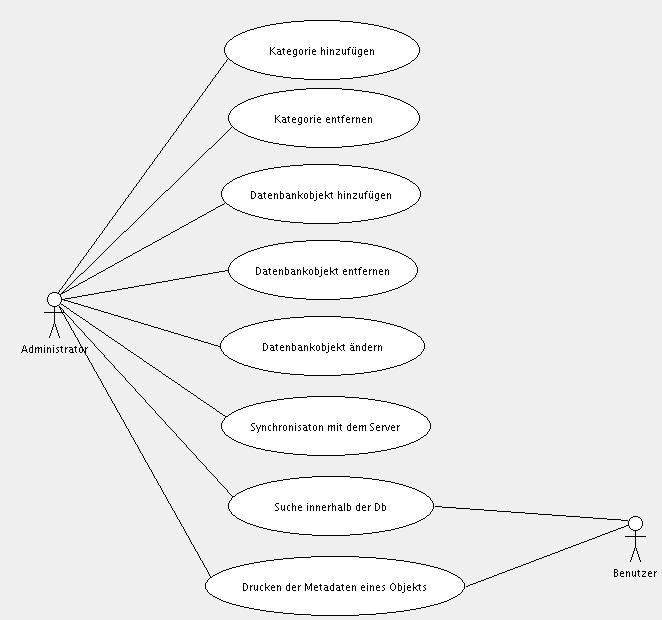
\includegraphics[scale=0.6]{images/Usecase.jpg}
                        \end{center}
                        \caption{Anwendungsf\"alle}
                        \label{fig:Usecase}
                    \end{figure*}\par


      Abbildung \ref{fig:Usecase} zeigt die Anwendungsf\"alle f\"ur die beiden Benutzergruppen. Es folgt eine textuelle
      Kurzbeschreibung der einzelnen F\"alle:

      \begin{enumerate}
        \item Kategorie \index{Kategorie}hinzuf\"ugen
            \begin{itemize} 
          \item Akteur: Administrator
          \item Vorbedingung: gew\"unschte Kategorie ist nicht in Kategorienliste enthalten
          \item Nachbedingung: Kategorienliste wird um die neue Kategorie erweitert
          \item Ablauf: Der Akteur gibt in einem Dialog den Name der neuen Kategorie an
            \end{itemize}
         
         \item Kategorie entfernen
            \begin{itemize}
                  \item Akteur: Administrator
                  \item Vorbedingung: der zu entfernenden Kategorie ist kein Objekt \index{Objekt} zugeordnet
                  \item Nachbedingung: Kategorie wird aus der Kategorienliste entfernt
                  \item Ablauf: Der Akteur w\"ahlt aus der ihm angezeigten Liste die betreffende Kategorie
          \item Fehlersituation: die zu entfernende Kategorie ist nicht leer, ein Entfernen ist nicht m\"oglich
                \end{itemize}

         \item Datenbankobjekt hinzuf\"ugen
             \begin{itemize}
                  \item Akteur: Administrator
                  \item Vorbedingung: keine
                  \item Nachbedingung: Objekt wird in die Datenbank aufgenommen
                  \item Ablauf: Der Aktuer w\"ahlt die entsprechende Objektart und die gew\"unschte Kategorie aus. 
            Er gibt anschlie{\ss}end die ben\"otigten Metadaten des Objekts ein.
                \end{itemize}

          \item Datenbankobjekt entfernen
          \begin{itemize}
                  \item Akteur: Administrator
                  \item Vorbedingung: zu entfernendes Objekt existiert in der Datenbank
                  \item Nachbedingung: Objekt wird aus Datenbank entfernt
                  \item Ablauf: Der Akteur sucht das entsprechende Objekt in der Datenbank und kann es dann
            entfernen
                \end{itemize}

          \item Datenbankobjekt \"andern
                  \begin{itemize}
                  \item Akteur: Administrator
                  \item Vorbedingung: zu \"anderdes Objekt existiert in der Datenbank
                  \item Nachbedingung: Metadaten \index{Metadaten} des entsprechenden Objekts werden ge\"andert
                  \item Ablauf: Der Akteur sucht das entsprechende Objekt in der Datenbank und kann dann die
            gew\"unschten \"Anderungen der Metadaten vornehmen.
                \end{itemize}

          \item Synchronisation \index{Synchronisation}mit dem Server
                  \begin{itemize}
                  \item Akteur: Administrator
                  \item Vorbedingung: keine
                  \item Nachbedingung: die neuen Eintr\"age werden dem Server \"ubermittelt und im Gegenzug neue 
            Servereintr\"age dem Client
                  \item Ablauf: Der Akteur w\"ahlt aus der ihm vorliegenden Serverliste den entsprechenden Server und kann
            sich dann mit ihm synchronisieren.
          \item Fehlersituation: Der Akteur hat keine administrativen Rechte auf dem gew\"ahlten Server.
                \end{itemize}

          \item Suchen innerhalb der Datenbank
                  \begin{itemize}
                  \item Akteure: Administrator, Benutzer
                  \item Vorbedingung: keine
                  \item Nachbedingung: keine
                  \item Ablauf: Der Akteur kann anhand eines Suchbegriffs aus den Metadaten Objekte suchen
          \item Fehlersituation: Der Suchbegriff konnte nicht in der Datenbank gefunden werden.
                \end{itemize}

          \item Drucken der Metadaten eines Objekt
                  \begin{itemize}
                  \item Akteure: Administrator, Benutzer
                  \item Vorbedingung: zu druckendes Objekt wurde ausgew\"ahlt
                  \item Nachbedingung: keine
                  \item Ablauf: Der Akteur kann das zur Zeit ausgew\"ahlte Objekt ausdrucken lassen
                \end{itemize}

      \end{enumerate}







        \section{Pflichtenheft}%Thorsten    
    Das hier dargestellte Pflichtenheft \index{Pflichtenheft}orientiert sich an den Vorgaben des 
    Buches ``Lehrbuch f\"ur Software-Technik'' von Helmut Balzert \cite{balzert}.

    \subsection{Zielbestimmungen}
       Unser Auftraggeber soll durch das Produkt in der Lage sein, seinen Literaturbestand effizient zu verwalten.
       
       \subsubsection{Mu{\ss}kriterien}
          \begin{itemize}
        \item Hinzuf\"ugen und Entfernen von Objekten \index{Objekt} zum Bestand
        \item Als Objekte gelten \index{Buch}B\"ucher, \index{Zeitschrift}Zeitschriften, Artikel, Audio- und Filmdateien
        \item Kategorisierung \index{Kategorie} des Bestands
        \item Suchfunktion anhand von Metadaten \index{Metadaten}
        \item Druckfunktion auf einem Postscript-Drucker \index{Drucker} \index{Postscript}
        \item Web-Client zum Durchsuchen der Datenbank mittels WWW \index{World Wide Web (WWW)}
      \end{itemize}
    \subsubsection{Wunschkriterien}
       \begin{itemize}
         \item Volltextsuche
         \item Import von anderen Datenformaten
         \item Export im BibTeX-Format \index{BibTeX}
         \item Hinzunahme weitere Objektarten bei Bedarf
       \end{itemize}

    \subsubsection{Abgrenzungskriterien}
       Obwohl f\"ur betriebsfremde Personen eine Ausleihm\"oglichkeit besteht, wird eine Ausleihverwaltung
       nicht realisiert.

    \subsection{Produkteinsatz}
       Das Produkt dient zur Verwaltung des gesamten Literaturbestands. Einzelne Mitarbeiter k\"onnen ihren
       individuellen Bestand pflegen und in den Gesamtbestand einflie{\ss}en lassen. Dieser kann von jedem
       Angestellten durchsucht werden, um den Standort des gesuchten Objekts ausfindig zu machen. Weiterhin
       ist es betriebsfremden Personen gestattet, die Datenbank mittels eines Web-Clients \"uber das WWW
       zu durchsuchen.

    \subsection{Produktumgebung}
       Das Produkt unterliegt einer Client-Server Architektur.\index{Client-Server Architektur}

       \subsubsection{Software}
          \begin{itemize}
             \item Betriebssystem: jedes, auf dem eine ``Sun Microsystems Java Runtime Engine'' lauff\"ahig ist \index{Java}

         \item Sonstige Software: Sun Microsystems \index{Sun Microsystems}Java Runtime Engine 
           (mindestens Version 1.4), eXist XML Datenbank
      \end{itemize}
       
       \subsubsection{Hardware}
          Sowohl der Server als auch jeder Client ben\"otigt lediglich die Hardware, die n\"otig ist, obige
      Software-Kriterien zu erf\"ullen. F\"ur die Verbindung von Server und Clients wird ein TCP/IP-Netzwerk
      ben\"otigt. \index{TCP/IP}

    \subsection{Produktfunktionen}
       \begin{enumerate}
     \item Verwaltung von Benutzergruppen mit Passw\"ortern \index{Passwort}
     \item Passwortabfrage beim Start des Programms
     \item Hinzuf\"ugen und Enfernen von Kategorien \index{Kategorie}
     \item Hinzuf\"ugen eines Objekts \index{Objekt}
       \begin{enumerate}
         \item Bestimmung der Objektart durch den Benutzer
         \item Bestimmung der Kategorie des Objekts durch den Benutzer
         \item Eingabe der ben\"otigten Metadaten durch den Benutzer
         \item Erzeugung einer eineindeutigen Signatur f\"ur das Objekt mit Hilfe der Kategorie durch das System
         \item Speicherung des Objekts in der Datenbank
       \end{enumerate}
     \item Entfernen eines Objekts
     \item Suchen eines Objektes anhand von Metadaten \index{Metadaten}
     \item \"Andern der Metadaten eines Objekt
     \item \"Ubermittlung der Daten des  pers\"onlichen Bestands an den Server (``Synchronisation'')\index{Synchronisation}
     \item Auswahl verschiedener Datenbankserver f\"ur den individuellen Gebrauch
     \item Erstellen einer Individualliste aus allen Datenbanken, die dem Benutzer zur Verf\"ugung stehen 
       \index{Individualliste}
         \item Drucken der Metadaten eines Objekts
         \item Import anderer Datenformate (insb. Excel)
         \item Export im BibTeX-Format \index{BibTeX}


       \end{enumerate}

    \subsection{Produktdaten}
       Alle Objektdaten werden im XML-Format gespeichert und halten sich so weit wie m\"oglich an die Vorgaben des 
       \index{Dublin Core} Dublin Core (vergl. \ref{dublin}). 

      


    \subsection{Benutzungsoberf\"ache} 
       Bei der Gestaltung der Benutzungsoberfl\"ache wird dem Entwicklungsteam 
       grunds\"atzlich freie Hand gelassen. \index{Oberfl\"ache, grafisch}
       Gefordert ist lediglich eine men\"uorientierte graphische Benutzungsoberfl\"ache (GUI), die haupts\"achlich 
       mit der Maus zu bedienen ist, trotzdem auch ohne Maus bedienbar bleibt. Durch die evolution\"are 
       Softwareentwicklung \index{Softwareentwicklung, evolution\"are} kann der erstellte und immer wieder 
       aktualisierte Prototyp \index{Prototyp} dem Auftraggeber zur Ansicht
       vorgelegt werden und so die Oberf\"ache st\"andig nach seinen W\"unschen verbessert werden.

    \subsection{Entwicklungsumgebung}

       \subsubsection{Software} \label{software}
          \begin{itemize}
        \item Als Programmiersprache wird Java \index{Java}verwendet. Ben\"otigt wird das ``Java Development Kit'' der Firma
          Sun Microsystems\footnote{\url{http://java.sun.com}} (mindestens Version 1.4).\index{Sun Microsystems}
        \item Als Programmierumgebung wird ``Eclipse'' von der Eclipse Foundation \index{Eclipse}
          empfohlen\footnote{\url{http://www.eclipse.org}}. Die Benutzung ist jedoch nicht zwingend.
        \item Als XML-Datenbank wird die Open-Source Datenbank ``eXist'' \index{Open-Source} \index{eXist}
          eingesetzt\footnote{\url{http://exist.sourceforge.net}}.
        \item Das Projekt betreffende Dokumente werden mit \LaTeX\ erstellt. \index{\LaTeX}
        \item Zum Versionsmanagement und zur Zusammenarbeit der beteilligten Entwickler wird CVS (Concurrent Version
          System) benutzt\footnote{\url{http://www.cvshome.org}}. \index{cvs}
      \end{itemize}

    \subsubsection{Hardware}
       Grunds\"atzlich wird keine spezielle Hardware erforderlich. Einziger Anspruch an die Hardware ist, dass die
       unter \ref{software} aufgef\"uhrten Programme und Werkzeuge einsetzbar sind.




